\documentclass{beamer}
\usetheme{Singapore}
\usecolortheme{default}

\usepackage[utf8]{inputenc}
\usepackage[T1]{fontenc}
\usepackage{verbatim}
\usepackage{graphics}

\title{Understanding Git with Alloy}
\author{Cláudio Lourenço \and Renato Neves}
\institute{University of Minho\\
Formal Methods in Software Engineering}


\logo{ 
\includegraphics[width=0.15\textwidth]{images/csail_logo.png}
       
\includegraphics[width=0.15\textwidth]{images/uminho_eng_logo.png}}
\begin{document}

\frame {
   \titlepage
}

\frame{
  \tableofcontents 
}

\section{Git in a hurry}
\frame{
   \frametitle{Introducing Git}
   \begin{block}{Distributed Version Control System}
      \begin{itemize}
         \item Records changes on files over time  %progit 2.1 
         \item Recall old versions of files
         \item Each client has a mirror of the repository %progit 2.1.3
      \end{itemize}
   \end{block}
   \begin{block}{Main differences with others VCS}
      \begin{itemize}
         \item Snapshots, Not Differences
      \end{itemize}
   \end{block}
}

\frame{
   \frametitle{The Git Object Model}
   \begin{minipage}
      \begin{figure}
         \centering
         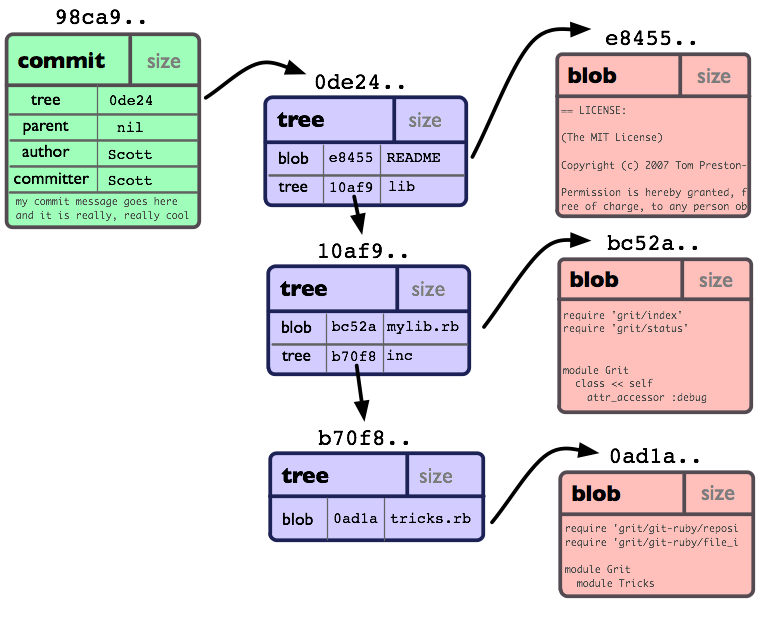
\includegraphics[width=0.55\textwidth]{images/object_model.png}
      \end{figure}
   \end{minipage}
   \begin{minipage}
      \begin{itemize}
         \item dasdsa
         \item dasdsa
      \end{itemize}
   \end{minipage}
}

\frame{
   \frametitle{Git workflow }
   \begin{figure}
      \centering
      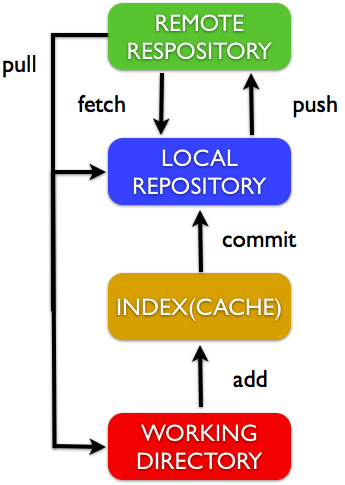
\includegraphics[width=0.35\textwidth]{images/data_flow_simplified.png}
   \end{figure}
   
}

\section{Project Goals}
\frame{
   \frametitle{Project Goals}
   \begin{itemize}
      \item Build a precise model of how Git works
      \item Analyze the model
      \item Check which properties the model (not) guarantee
      \item Compare to other systems
      \item Build a concise user manual based on the model
   \end{itemize}
}

\section{Progress so far}
\frame{
   \frametitle{What has been done so far}
   \begin{block}{First Approach}
      \begin{itemize}
         \item Model Working Directory
         \item Model Index
         \item Model Object Model
         \begin{itemize}
            \item Object hash are modeled
         \end{itemize}
      \end{itemize}
   \end{block}
   \begin{block}{Problem}
      \begin{itemize}
         \item Model got too complex when adding operations
      \end{itemize}
   \end{block}
}

\frame{
   \frametitle{What has been done so far}
   INSTANCIA
}

\frame{
   \frametitle{What has been done so far}
   \begin{block}{Second Approach}
      \begin{itemize}
         \item Focus on Object Model and Index
         \item Files are just a set of paths
         \item Object hash are the alloy atom's name
      \end{itemize}

   \end{block}
}


\frame{
   \frametitle{What has been done so far}
   INSTANCIA
}

\frame{
   \titlepage
}

\end{document}
